\documentclass[12pt]{article}
\usepackage[utf8]{inputenc}
\usepackage[T1]{fontenc}
\usepackage[ngerman]{babel}
\usepackage{amsmath, amssymb, amsfonts, graphicx, hyperref, geometry, parskip, listings, caption}
\usepackage{breqn}
\usepackage{float}
\usepackage{color} % For listings syntax highlighting
\geometry{a4paper, margin=2.5cm}
\lstset{
    language=Python,
    basicstyle=\ttfamily\scriptsize,
    keywordstyle=\color{blue},
    stringstyle=\color{red},
    commentstyle=\color{green!60!black},
    showstringspaces=false,
    breaklines=true,
    breakatwhitespace=true,
    frame=single,
    xleftmargin=2mm,
    xrightmargin=2mm
}
\hyphenation{Uni-ver-sal Re-so-nance Mas-ter Equa-tion quan-tum-clas-si-cal hy-brid sys-tems Ap-pli-ca-tion Ca-te-go-ries for-mer-ly se-pa-rate equa-tions Uni-ver-sel-len Re-so-nanz-Mas-ter-gleich-ung quan-ten-klas-sis-chen Hy-brid-sys-te-men}

\title{\textbf{Resonanz-Mastergleichung -- Schlüssel zu neuen Dimensionen}}
\author{Adrian Zander -- \href{mailto:zander.adrian@gmx.de}{zander.adrian@gmx.de}}
\date{\today}

\begin{document}
\maketitle

\begin{sloppypar}
Dieses Whitepaper präsentiert ein modulares und einheitliches Framework zur Modellierung physikalischer Systeme durch die Linse der Resonanz. Durch die Einführung der Universellen Resonanz-Mastergleichung kapseln wir vielfältige Phänomene ein, die von klassischer Gitterdynamik bis hin zu quanten-klassischen Hybridsystemen reichen.
\end{sloppypar}

\clearpage

\section*{Einleitung}
Das Universelle Resonanzmodell (URM) postuliert, dass alle physikalischen Phänomene als Netzwerke gekoppelter Oszillationen verstanden werden können. Dieses Dokument liefert die mathematisch-physikalischen Grundlagen sowie entsprechende numerische Simulationsstrategien in Python.

\section*{Universelle Resonanz-Mastergleichung}
\begin{dmath}
m \ddot{x}_{i,j} = k \Delta x_{i,j} - c \dot{x}_{i,j} - \alpha x_{i,j}^3 - \beta x_{i,j}^5 + q E_{i,j}(t) + \lambda \langle \hat{Q}_{i,j} \rangle + \gamma X_{i,j}(t) + \eta T_{i,j} + \xi \zeta_{i,j}(t) + F_{i,j}(t)
\end{dmath}

\subsection*{Bedeutung der Terme}
\begin{itemize}
\item $\Delta x_{i,j}$: Diskreter Laplace-Operator (Gitterkopplung)
\item $\alpha, \beta$: Nichtlinearitäten (kubisch, quintisch)
\item $E_{i,j}(t)$: Externes klassisches Feld (z.B. elektromagnetisch)
\item $\langle \hat{Q}_{i,j} \rangle$: Quantenerwartungswert
\item $X_{i,j}(t)$: Makroskopische Kopplung (z.B. mittlere Feldamplitude)
\item $T_{i,j}$: Topologischer Term (z.B. lokale Defekte)
\item $\zeta_{i,j}(t)$: Stochastisches Rauschen
\item $F_{i,j}(t)$: Externe Anregung (z.B. sinusförmige Kraft)
\end{itemize}

\clearpage

\section*{Python: Modulare Simulationsvorlage}
\begin{lstlisting}[language=Python]
def external_field(i, j, t):
    return np.sin(0.1 * i + t)

def quantum_expectation(i, j, t):
    return np.sin(0.05 * i * j + t)

def macro_resonance(x):
    return np.mean(x)

def topological_term(i, j, x, N):
    term1 = abs(x[i, j] - x[(i + 1) % N, j])
    term2 = abs(x[i, j] - x[i, (j + 1) % N])
    return term1 + term2

def stochastic_noise():
    return np.random.normal(0, 1)
\end{lstlisting}

\clearpage

\section*{\small Anwendungskategorien (ehemals separate Gleichungen)}

\subsection*{RNLE -- Resonante Nichtlineare Gittergleichung}
$-\alpha x^3, -\beta x^5$: Für klassische nichtlineare Festkörpermodelle.

\subsection*{FCLE -- Feld-gekoppelte Gittergleichung}
$+ q\, E_{i,j}(t)$: Kopplung an externe Felder.

\subsection*{MSCRE -- Multiskalige Gekoppelte Resonanz}
$+ \gamma\, X_{i,j}(t)$: Rückkopplung über makroskopische Resonanz.

\subsection*{QCRE -- Quanten-gekoppelte Resonanz}
$+ \lambda\, \langle \hat{Q}_{i,j} \rangle$: Hybrid Quanten-Klassik-Kopplung.

\subsection*{TRE -- Topologische Resonanzgleichung}
$+ \eta\, T_{i,j}$: Topologische Effekte (z.B. Kanten, Defekte).

\subsection*{DQRE / DDRE -- Dissipative Quanten-/Getriebene Resonanz}
$+ \xi\, \zeta_{i,j}(t)$: Stochastische oder Umwelteinflüsse.

\section*{Fazit}
Alle Spezialfälle werden durch die Wahl der Parameter in der Mastergleichung abgedeckt. Diese modulare Struktur ermöglicht eine effiziente und skalierbare Umsetzung zur Erforschung komplexer Oszillatornetzwerke.

\begin{figure}[H]
\centering
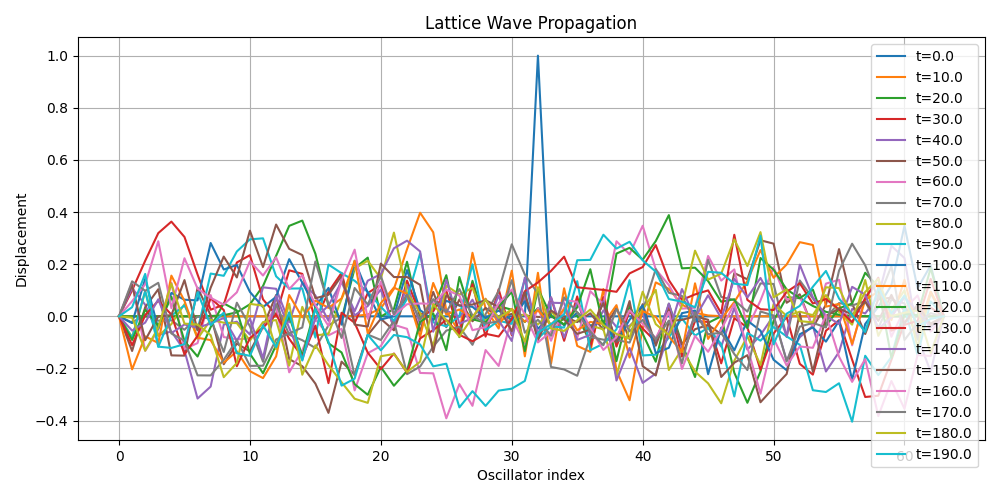
\includegraphics[width=0.8\textwidth]{lattice_wave_propagation.png}
\caption{Wellenpropagation im Gitter (Wave Propagation in the Lattice)}
\end{figure}

\begin{figure}[H]
\centering
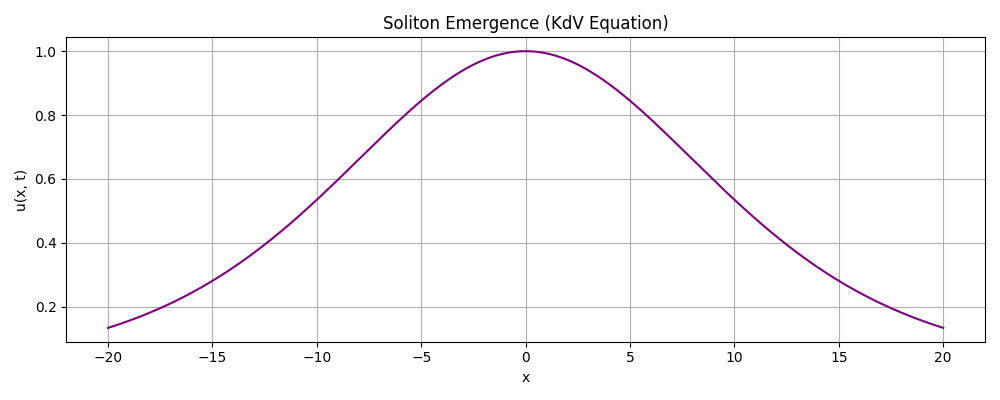
\includegraphics[width=0.8\textwidth]{soliton_emergence.png}
\caption{Solitonentstehung (Soliton Emergence)}
\end{figure}

\end{document}